\section{Markov Decision Process (MDP)}

\definecolor{darkgreen}{rgb}{0,0.6,0}

\begin{frame} 
\mode<presentation>{
    \begin{center} \huge
        \secname
    \end{center}
}
    \begin{center}
    A formalized description of the \underline{environment} in RL\footnote{Recommended reading 
\citep{sutton1998introduction} also video lectures by David Silver}
    \end{center}
\end{frame}


\begin{frame}\frametitle{\secname}
    
\begin{block}{Assumption of MDP}
The environment is fully observable. There is a complete characterization of what's going on and where everything is.
\end{block}

The other case would be \emph{partially observable} MDP (POMDP)

\end{frame}


\begin{frame}\frametitle{\secname}

\begin{block}{What do we want to do?}
Maximize, not just immediate rewards, but the \emph{cumulative sum of rewards} or ``return''.
\slidesonly{\vspace{-3mm}}
\begin{equation}
\mathit{return}(t) := \sum_{k=0}^{\infty} \gamma^k r(\vec x^{(t+k+1)}, \vec a^{(t+k+1)}) = \sum_{k=0}^{\infty} \gamma^k r^{(t+k+1)},
\end{equation}

where $\gamma \in \lbrack0,1)$ is referred to as the \emph{discount factor}.
 
\end{block}

\only<1,2>{
About the \emph{discount factor} $\gamma$:
}

\begin{itemize}
\only<1,2>{
\item It is possible for $\gamma$ to be $=1$.\\

\pause
	
\question{Under what condition can $\gamma$ be $=1$}\\

\pause

\begin{center}
	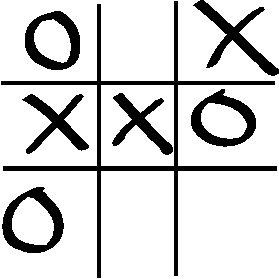
\includegraphics[width=0.2\textwidth]{img/tic-tac-toe}
	\mode<article>{
	\captionof{figure}{Some games can always be completeted in a finite number of steps.}
	}
\end{center}


\mode<article>{
- $\gamma$ can be $=1$ if the length of the sequence is guaranteed to be finite.
}
}

\pause

\item \question{What does $\gamma \rightarrow 0$ imply?}\\

\pause

\pause

- preference for short term rewards

\pause

\item \question{What does $\gamma \rightarrow 1$ imply?}\\

\pause

- emphasis on long-term returns, indifference to delay.

\end{itemize}

\end{frame}

\begin{frame}\frametitle{The discount factor}
 
\mode<presentation>{
\begin{equation}
\mathit{return}(t) := \sum_{k=0}^{\infty} \gamma^k r^{(t+k+1)},\quad \text{where }\gamma \in \lbrack0,1)
\end{equation}

}

\mode<article>{
\figref{fig:discount} illustrates how the choice of $\gamma$ controls how fast the discount factors decay over time.
}

\begin{center}
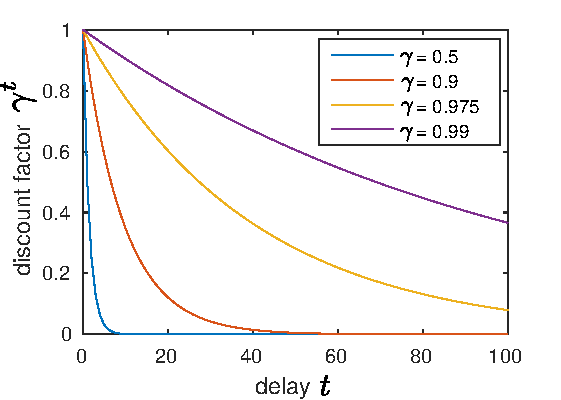
\includegraphics[width=6cm]{img/delay_discount}
\captionof{figure}{modulating returns with different discount factors}
\label{fig:discount}
\end{center}

\slidesonly{\vspace{-3mm}}
%\slidesonly{\textbf{(see blackboard)}}

\end{frame}

\newpage

\begin{frame}{Example: big reward further away vs. closer smaller reward}

\mode<article>{


\textbf{Example}: big reward further away vs. closer smaller reward\\

\figref{fig:mouse_walk}) illustrates a simple environment. The mouse can move one tile at a time to the \textbf{R}ight or to the \textbf{L}eft. We'll compare the return of two different strategies for different discount factors.
}

\mode<presentation>{
\begin{equation}
\mathit{return}(t) := \sum_{k=0}^{\infty} \textcolor{magenta}{\gamma}^k r^{(t+k+1)}
\end{equation}

}

\begin{center}
\only<-2,7->{
	
\includegraphics[width=8cm]{img/mouse_walk_wide}
}
\only<3-6>{
	\slidesonly{
	\svspace{-3mm}
		
\includegraphics[width=8cm]{img/mouse_walk_wide_steps}	
	\svspace{-3mm}
	}	
}
	\notesonly{\captionof{figure}{Environment with two rewards placed at different distances from the initial position of the mouse.}}
	\label{fig:mouse_walk}
\end{center}

\pause

\mode<presentation>{
Comparing two strategies under different discount factors:

\begin{itemize}
\item $\longrightarrow$,$\longrightarrow$,$\longrightarrow$,\ldots\\
\only<3->{
	\begin{itemize}
		\item[] $\scriptstyle \textcolor{magenta}{\gamma=0.7}:~$ $\scriptstyle \mathit{return}(0)=
		\only<4->{
		0.7^0\cdot~0~+~0.7^1\cdot~0~+~
		}
		\only<5>{
		0.7^2\cdot~1~+~
		}
		\only<6->{
		0.49~\cdot~1~+~0.7^3 \cdot~0~+~\ldots~\ge~0.49
		}
		$
	\only<10->{
		\item[] $\scriptstyle \textcolor{magenta}{\gamma=0.2}:~$ $\scriptstyle \mathit{return}(0)=
		\only<11>{
		1~\cdot~0~+0.2~\cdot~0~+~0.2^2~\cdot~1~+~\ldots~\ge~\mathbf{0.04}
		}
		$
	}
	\end{itemize}
}
\item $\longleftarrow$,$\longleftarrow$,$\longleftarrow$,\ldots\\
\only<7->{
	\begin{itemize}
		\item[] $\scriptstyle \textcolor{magenta}{\gamma=0.7}:~$ $\scriptstyle \mathit{return}(0)=
		\only<7->{
		0.7^0\cdot~0~+~0.7^1\cdot~0~+~
		}
		\only<8->{
		0.7^2\cdot~0~+~
		}
		\only<9->{
		0.7^3\cdot~3~+~\ldots~\ge~\mathbf{1.029}
		}
		$
	\only<10->{
		\item[] $\scriptstyle \textcolor{magenta}{\gamma=0.2}:~$ $\scriptstyle \mathit{return}(0)=
		\only<11>{
		1~\cdot~0~+0.2~\cdot~0~+~0.2^2~\cdot~0+~0.2^3~\cdot~3~+~\ldots~\ge~0.024
		}
		$
	}
	\end{itemize}
}
\end{itemize}
}

\mode<article>{
% Please add the following required packages to your document preamble:
% \usepackage{graphicx}
\begin{table}[h]
\centering
\resizebox{0.7\textwidth}{!}{%
\begin{tabular}{lcrl}
\multicolumn{1}{c|}{strategy}   & \multicolumn{1}{c|}{$\gamma$}                       & $\mathit{return}(0)$                                                                  &                                                 \\ \hline \hline
                                %& \multicolumn{1}{l}{}                                & \multicolumn{1}{l}{}                                                       &                                                 \\ \hline
%\multicolumn{1}{|c|}{strategy}  & \multicolumn{1}{c|}{$\gamma$}      & return(1)                                                                  & \multicolumn{1}{l|}{}                           \\ \hline \hline
                                %& \multicolumn{1}{l}{}               & \multicolumn{1}{l}{}                                                       &                                                 \\ \hline
\multicolumn{1}{|l|}{R,R,...}   & \multicolumn{1}{c|}{\multirow{2}{*}{$\frac{1}{2}$}} & $1 \cdot 0 + \frac{1}{2} \cdot 0 + \frac{1}{4} \cdot 1 + \ldots$                       & \multicolumn{1}{l|}{$\ge {0.25}$}             \\   \cline{1-1} \cline{3-4}
\multicolumn{1}{|l|}{L,L,L,...} & \multicolumn{1}{c|}{}              & $1 \cdot 0 + \frac{1}{2} \cdot 0 + \frac{1}{4} \cdot 0 + \frac{1}{8} \cdot 3 + \ldots$ & \multicolumn{1}{l|}{$\ge \mathbf{0.375}$} \\ \hline
                                & \multicolumn{1}{l}{}               & \multicolumn{1}{l}{}                                                       &                                                 \\   \hline
\multicolumn{1}{|l|}{R,R,...}   & \multicolumn{1}{c|}{\multirow{2}{*}{$0.7$}}         & $1 \cdot 0 + 0.7 \cdot 0 + 0.7^2 \cdot 1 + \ldots$                                     & \multicolumn{1}{l|}{$\ge {0.49}$}                 \\ \cline{1-1} \cline{3-4}
\multicolumn{1}{|l|}{L,L,L,...} & \multicolumn{1}{c|}{}         & $1 \cdot 0 + 0.7 \cdot 0 + 0.7^2 \cdot 0 + 0.7^3 \cdot 3 + \ldots$                     & \multicolumn{1}{l|}{$\ge \mathbf{1.029}$}                 \\ \hline
                                & \multicolumn{1}{l}{}               & \multicolumn{1}{l}{}                                                       &                                                 \\ \hline
\multicolumn{1}{|l|}{R,R,...}   & \multicolumn{1}{c|}{\multirow{2}{*}{$0.2$}}         & $1 \cdot 0 + 0.2 \cdot 0 + 0.2^2 \cdot 1 + \ldots$                                     & \multicolumn{1}{l|}{$\ge \mathbf{0.04}$}                  \\   \cline{1-1} \cline{3-4}
\multicolumn{1}{|l|}{L,L,L,...} & \multicolumn{1}{l|}{}              & $1 \cdot 0 + 0.2 \cdot 0 + 0.2^2 \cdot 0 + 0.2^3 \cdot 3 +\ldots$              & \multicolumn{1}{l|}{$\ge {0.024}$}                \\ \hline
\end{tabular}%
}
\captionof{table}{Comparing returns under different discount factors.}

\end{table}
}

\end{frame}

\begin{frame}

\question{Why do we discount future rewards? What criteria go into choosing $\gamma$?}\\

\pause

\begin{itemize}
\item Uncertainty of the future
\item Imperfections in the model (we don't trust its decisions completely)
\item mathematically convenient, the sum does not explode
\item avoids $\infty$ returns due to possible cycles in our MDP
\item behavioral arguments (animals and humans seem to apply a similar discounting)\\
``A bird in the hand is worth two in the bush''
\item financially realistic (accounts for inflation)
\end{itemize}

\end{frame} 

\newpage

\subsection{The value function}


\definecolor{darkgreen}{rgb}{0,.5,0}
\definecolor{discount}{rgb}{.75,0,.75}
\definecolor{expect}{rgb}{0,.5,.5}
\definecolor{chain}{rgb}{.75,.5,0}

\begin{frame}\frametitle{\subsecname}

The (state) value function $\corresponds$ the expected sum of discounted future rewards

\question{What does the value function represent?}

\begin{itemize}
\item The long-term value of some state $\vec x$,
\item the expected return from starting in $\vec x^{(0)}$,
\item we have a preference for high expectations and MDPs maximize this quantity
\end{itemize}

\end{frame}

\begin{frame}\frametitle{\subsecname}

\mode<presentation>{
The value function $\corresponds$ the expected sum of discounted future rewards
}

For a fixed policy ${\color{policy}\pi}$:

	\only<1-4>{
	
	\begin{itemize}
		\item a \textbf{value function} measures the quality 
			of a policy $\pi$ in state $\vec x^{(0)}$
			\iitem{$V^\pi(\vec x^{(0)})$ is
				the {\em \visible<1->{{\color{expect}expected}} 
				\visible<2->{{\color{chain}{%
						\only<3>{\color{discount}}%
						\visible<3->{infinite} 
					}sum} of}
				\visible<3->{{\color{discount} discounted}} 
				\visible<2->{future}
				\visible<1->{{\color{reward}reward\visible<2->{s}}}}}
	\end{itemize}
	\only<1,3>{\vspace{1mm}}
	
	\begin{equation}
				V^\pi(\vec x^{(0)}) 
				\;\;=\;\; \visible<1->{{ \color{expect}	\E\bigg\lbrack }} 
					\visible<2->{{\color{chain}\sum_{t=0}^{
						\slidesonly{\only<2>{H}}%
						\only<3->{{\color{discount}\infty}}}}}
				\visible<3->{{\color{discount} \gamma^t} \,}
				{\color{reward} r(
					\slidesonly{\only<1>{{\color{black} \vec x^{(0)}}}}
					\only<2->{{\color{trans} \vec x^{(t)}}}, 
					{\color{policy}\vec a^{(\slidesonly{\only<1>{0}}\only<2->{t})}}
				) } 
				{ \color{expect}
					\,\bigg| \begin{array}{c}
							\scriptstyle {\color{policy}
								\vec a^{(\slidesonly{\only<1>{0}}\only<2->{t})} 
								\;\sim\; \pi(\cdot\,|\,
									\vec x^{(\slidesonly{\only<1>{0}}\only<2->{t})}) 
								}\;\;\;\\
							\visible<2->{{\color{trans}
								\scriptstyle \vec x^{(t+1)} \;\sim\; 
								P(\cdot \,|\, \vec x^{(t)}, \vec a^{(t)})
							}}
					\end{array}\kern-1ex 
					\bigg\rbrack
				} 
				\visible<3->{\,,\quad {\color{discount}\gamma \in \lbrack0, 1)} \,.}
	\end{equation}
	}
    \only<5>{
    \mode<presentation>{
    \begin{center}
		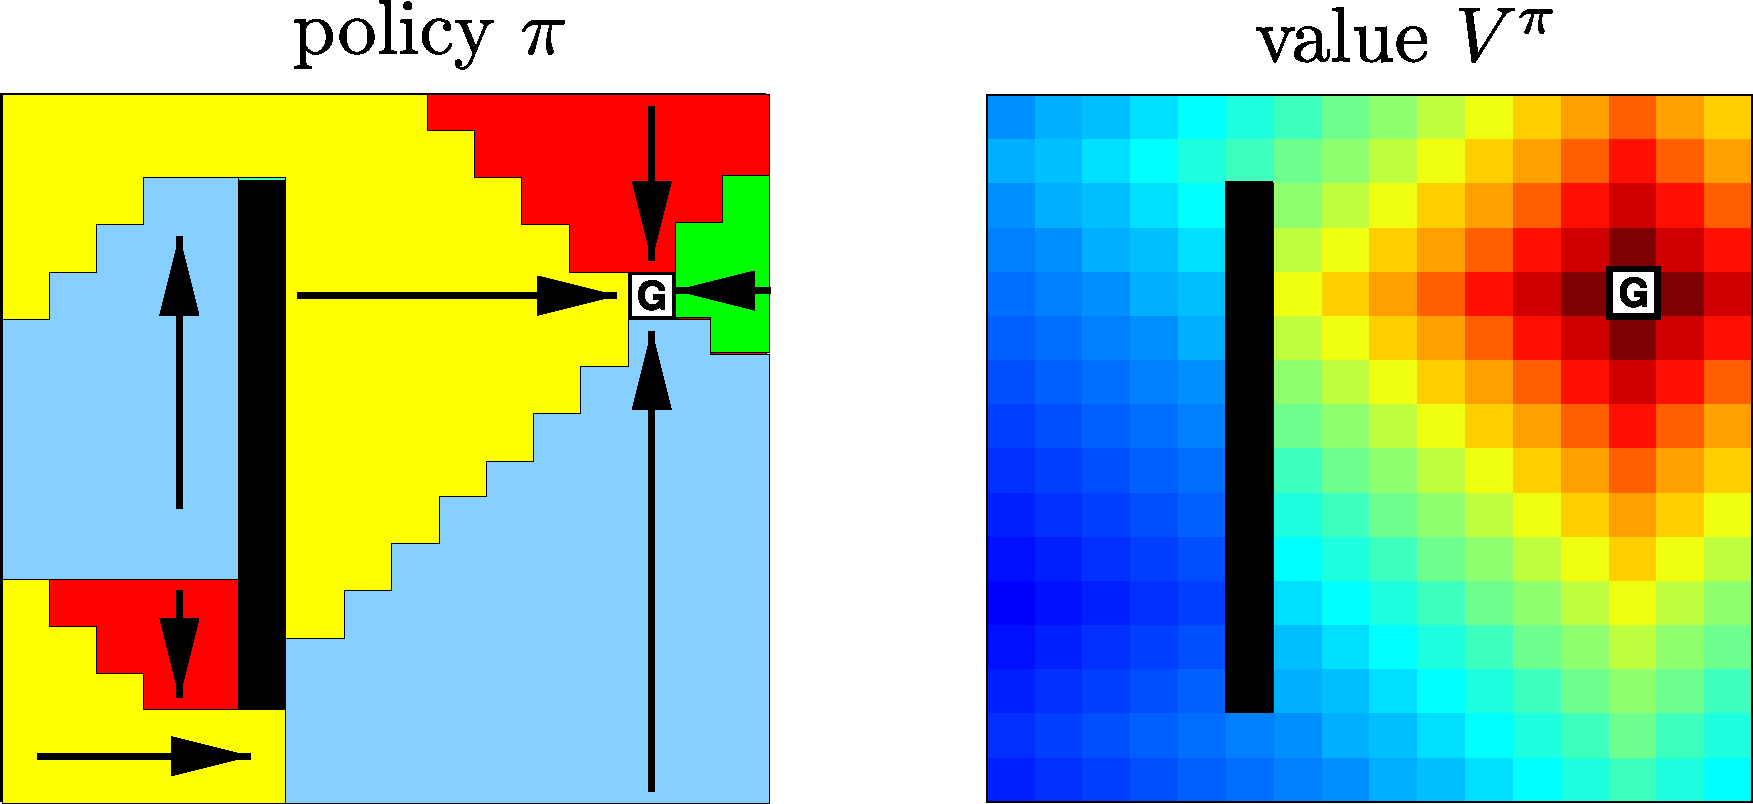
\includegraphics[trim={15cm 0 0 0mm},clip, height=3.cm]{img/nav_policy_and_value}
	\end{center}
    }
    }
    
    \visible<4,5>{
    
    
	In other textbooks you may find:
	
	\begin{align}
	V^\pi(\vec x_i) = \kern-1ex \overbrace{V^\pi_i}^{\text{shorthand}} \kern-1ex = 
	\E \bigg\lbrack
	\sum_{t=0}^{\infty} \gamma^t r(\vec x^{(t)}, \vec a^{(t)}) \;\Big|\; \vec x^{(0)} := \vec x_i
	\bigg\rbrack\,, \; i=1,\ldots,S
	\end{align}
	
	$\E\lbrack\cdot\rbrack$ is w.r.t $\{\vec x^{(t)}, \vec a^{(t)}\}$

    }

\end{frame}
